% This work is licensed under the Creative Commons Attribution-NonCommercial 4.0 International License.
% To view a copy of this license, visit http://creativecommons.org/licenses/by-nc/4.0/
% or send a letter to Creative Commons, PO Box 1866, Mountain View, CA 94042, USA.

% !TEX TS-program = xelatex

\documentclass[../Main/chem532-notes.tex]{subfiles}

\begin{document}

\chapter[The molecular Hamiltonian]{The molecular Hamiltonian and the Born--Oppenheimer approximation}

\section{Atomic Units} 
For convenience, we define a set of \textbf{atomic units} (abbreviated a.u.) for which:
\begin{align}
\text{electron mass} & = m_e = 1\\
\text{electron charge} & = e = 1\\
\text{action} & = \hbar = \frac{h}{2\pi} = 1\\
\text{Coulomb's constant} & = k_e = \frac{1}{4\pi \epsilon_0} = 1
\end{align}

In atomic units:
\begin{table}[htbp]
\centering
\begin{tabular}{lll}
\toprule
Dimension & Symbol (Name) & Value in Other Units\\
\midrule
Length & $a_0$ (bohr) & 0.52918 \AA{} \\ 
Mass & $m_e$ & $9.1095 \times 10^{-31}$ Kg \\
Charge & $e$ & $1.6022 \times 10^{-19}$ C \\
Action & $\hbar$ & $1.05457 \times 10^{-34}$ J $\cdot$ s \\
%Coulomb's constant & $\frac{1}{4\pi \epsilon_0}$ & $ \times 10^{-34}$ J $\cdot$ s \\
Energy & $E_{\rm h}$ (Hartree) & 627.51 kcal/mol \\
& & 27.211 eV \\
& & 219474.63 cm$^{-1}$ \\
& & $4.3598 \times 10^{-18}$ J\\
Time & & $2.41889 \times 10^{-17}$ s $\approx 1/41.3$ fs\\
\bottomrule
\end{tabular}
%\caption{Remember, \emph{never} use vertical lines in tables.}
\label{tab:atomicunits}
\end{table}

The speed of light in atomic units is $\alpha^{-1}\approx 137$ a.u.\mnote{$\alpha$ is the fine-structure constant}

\section{The molecular Hamiltonian}
Consider a molecule containing $N$ electrons and $M$ nuclei.
We will indicate the position of the nuclei with $\vec{R}_A = \mathbf{R}_A = (X_A,Y_A,Z_A)$ and that of electrons with $\vec{r}_i = \mathbf{r}_i = (x_i,y_i,z_i)$.

\begin{table}[h!]
\caption{Symbols used in the definition of the molecular Hamiltonian [Eq.~\eqref{eq:molecular_hamiltonian}].}
\centering
\begin{tabular}{llllll}
\toprule
Particle & Number & Indices & Position & Mass & Charge\\
\midrule
Electrons & $N$ & $i, j, k, \ldots$ & $\vec{r}_i = (x_i,y_i,z_i)$ & $m_e = 1$ & $-e = -1$\\
Nuclei & $M$ & $A, B, C, \ldots$ & $\vec{R}_A = (X_A,Y_A,Z_A)$ & $M_A = M_A/m_e$ & $e Z_A = Z_A$\\
\bottomrule
\end{tabular}

%\label{tab:atomicunits}
\end{table}

The total Hamiltonian is given by
\begin{equation}
\hat{H} = \hat{T}_N + \hat{T}_e + \hat{V}_{NN} + \hat{V}_{eN} + \hat{V}_{ee},
\end{equation}
where
\begin{align}
\hat{T}_\mathrm{N} &= -\frac{\hbar^2}{2} \sum_A^M \frac{1}{M_A} \nabla^2_A, \\
\hat{T}_\mathrm{e} &= -\frac{\hbar^2}{2 m_e} \sum_i^N \nabla^2_i, \\
\hat{V}_\mathrm{NN} &= +\sum_{A}^{M} \sum_{B > A}^{M} \frac{1}{4 \pi \epsilon_0} \frac{e^2 Z_A Z_B}{r_{AB}}, \\
\hat{V}_\mathrm{eN} &= - \sum_{i}^{N} \sum_{A}^{M} \frac{1}{4 \pi \epsilon_0} \frac{e^2 Z_A}{r_{iA}}, \\
\hat{V}_\mathrm{ee} &= +\sum_{i}^{N}\sum_{j > i}^{N} \frac{1}{4 \pi \epsilon_0} \frac{e^2}{r_{ij}},
\end{align}
and the quantity $r_{ij}$ is the distance between electrons labeled with indices $i$ and $j$
\begin{equation}
r_{ij} = |\vec{r}_i - \vec{r}_j| = \sqrt{(x_i-x_j)^2 + (y_i-y_j)^2 + (z_i-z_j)^2},
\end{equation}
and $r_{iA} = |\vec{r}_i - \vec{R}_A|$ and $r_{AB} = |\vec{R}_A - \vec{R}_B|$ are defined similarly.

In atomic units the Hamiltonian is more compact:
\begin{equation}
\label{eq:molecular_hamiltonian}
\hat{H} =
-\frac{1}{2} \sum_A^M \frac{1}{M_A} \nabla^2_A
 -\frac{1}{2} \sum_i^N \nabla^2_i
+ \sum_{A}^{M} \sum_{B > A}^{M} \frac{Z_A Z_B}{r_{AB}}
- \sum_{i}^{N} \sum_{A}^{M} \frac{Z_A}{r_{iA}}
+ \sum_{i}^{N}\sum_{j > i}^{N} \frac{1}{r_{ij}},
\end{equation}
where $M_A$ is understood to be the mass of nucleus $A$ in atomic units.

If we define the collective electronic ($\mathbf{r} = \{ \vec{r}_i \}$) and nuclear ($\mathbf{R} = \{ \vec{R}_A \}$) degrees of freedom, we may write the Schr\"{o}dinger equation compactly as:
\begin{equation}
\hat{H} \Psi_k(\mathbf{r},\mathbf{R}) = E_k \Psi_k(\mathbf{r},\mathbf{R}).
\end{equation}

Note that $\Psi_k(\mathbf{r},\mathbf{R})$ is a complicated function of $3^{N+M}$ variables (excluding spin) because it depends both on the coordinate of the electrons and nuclei. For a free molecule it includes translational, rotational, vibrational, and electronic degrees of freedom.
The terms that make this Hamiltonian difficult to solve are those that couple electrons and nuclei, that is, $\hat{V}_\mathrm{NN}$, $\hat{V}_\mathrm{eN}$, and $\hat{V}_\mathrm{eN}$ is problematic because it couples electrons and nuclei.

\begin{problem}	
What does the spectrum of $\hat{H}$ look like for a diatomic molecule?
\end{problem}



\section{The Born--Oppenheimer approximation}
One way to simplify the molecular Hamiltonian is to recognize that since electrons and nuclei have very different masses (the lowest value that $M_A$ can have is 1837 $m_e$, for the hydrogen atom) and treat the electronic and nuclear degrees of freedom separately.
In the Born--Oppenheimer approximation we first solve the Schr\"{o}dinger equation for the electrons assuming that the nuclei are fixed in space ($\mathbf{R}$ is a constant).
To do so we define an \textbf{electronic} Hamiltonian ($\hat{H}_{\rm el}$):
\begin{equation}
\hat{H}_\mathrm{el} = \hat{T}_\mathrm{e} + \hat{V}_\mathrm{eN} + \hat{V}_\mathrm{ee},
\end{equation}
and seek its corresponding eigenvalues and eigenfunctions:
\begin{equation}
\hat{H}_\mathrm{el} \Phi_{\mathrm{el},k}(\mathbf{r};\mathbf{R})
= E_{\mathrm{el},k}(\mathbf{R}) \Phi_{\mathrm{el},k}(\mathbf{r};\mathbf{R}).
\end{equation}
Note that $\mathbf{R}$ enters these equations as a parameter, hence we use the symbol ``;'' to separate it from the variable $\mathbf{r}$. The different pairs of eigenvalues/eigenfunctions are labeled by the state index $k$ which can take the values 0, 1, \ldots. The state with $k = 0$ [$E_{{\rm el},0}(\mathbf{R})$] is called the \textbf{ground electronic state}, while states with $k > 0$ are \textbf{excited electronic states}.

When discussing the properties of molecules, it is convenient to refer to the total potential energy [$V_{k}(\mathbf{R})$] in the fixed nuclei approximation which includes the contribution of the nuclear-nuclear repulsion potential
\begin{equation}
V_{k}(\mathbf{R}) = E_{\mathrm{el},k}(\mathbf{R}) + \sum_{A}^{M} \sum_{B > A}^{M} \frac{Z_A Z_B}{r_{AB}}.
\end{equation}
This quantity is commonly known as the \textbf{potential energy surface} (abbreviates as PES).
Note that $V_{k}(\mathbf{R})$ gives us the potential energy at a given molecular geometry $\mathbf{R}$ and therefore it describes a set of surfaces in $3^M$ dimensions.

\begin{example}[Potential energy surface of H$_2^+$]
The following plot shows the contributions of the electronic energy ($E_\mathrm{el}$) and the nuclear repulsion energy ($V_\mathrm{NN}$) to the potential energy of the ground state of H$_2^+$.
\begin{center}
\includegraphics[width =5in]{../molecular-hamiltonian/h2+_pec.pdf}
\end{center}
\end{example}

Although there are $3M$ nuclear degrees of freedom (DOF), in absence of an external potential translations and rotations of a molecule do not change the value of $V_{k}(\mathbf{R})$. Therefore, the number of internal degrees of freedom that change the value of $V_{k}(\mathbf{R})$ is less than $3M$. For a non-linear molecule we have that
\begin{equation}
\text{internal DOF} = \underbrace{3 M}_{\text{total DOF}}
-\underbrace{3}_{\text{rotations}}
-\underbrace{3}_{\text{translations}} = 3M - 6,
\end{equation}
while for a linear molecule
\begin{equation}
\text{internal DOF} = \underbrace{3 M}_{\text{total DOF}}
-\underbrace{2}_{\text{rotations}}
-\underbrace{3}_{\text{translations}} =  3M - 5.
\end{equation}

\begin{example}[Diatomic molecule]
For a diatomic molecule there is $2\cdot3 - 5 = 1$ degrees of freedom. In this case $V_{k}(\mathbf{R})$ may be expressed in terms of the bond distance $R$ as $V_{k}(\mathbf{R})$. In this case we call these quantities \textbf{potential energy curves}.
\end{example}

The concept of the potential energy surface is at the basis of many concepts used to describe molecules like, the molecular geometry, transition states, etc.
The equilibrium geometry of a molecule in a given electronic state $k$, $\mathbf{R}_\mathrm{eq}$, is defined as the minimum of $V_{k}(\mathbf{R})$, that is, the gradient of $V_{k}(\mathbf{R})$ at this geometry is zero
\begin{equation}
\left. \frac{\partial V_{k}(\mathbf{R})}{\partial \mathbf{R}} \right|_{\mathbf{R}= \mathbf{R}_\mathrm{eq}}= 0,
\end{equation}
and the curvature of $V_{k}(\mathbf{R})$ at $\mathbf{R}_\mathrm{eq}$ is positive (the eigenvalues of the second derivative matrix or Hessian are all positive).
Note that for a given electronic state equilibrium geometry may be unique or not, and may not even correspond to a bound molecular state.



%\begin{figure}[htbp]
%   \centering
%   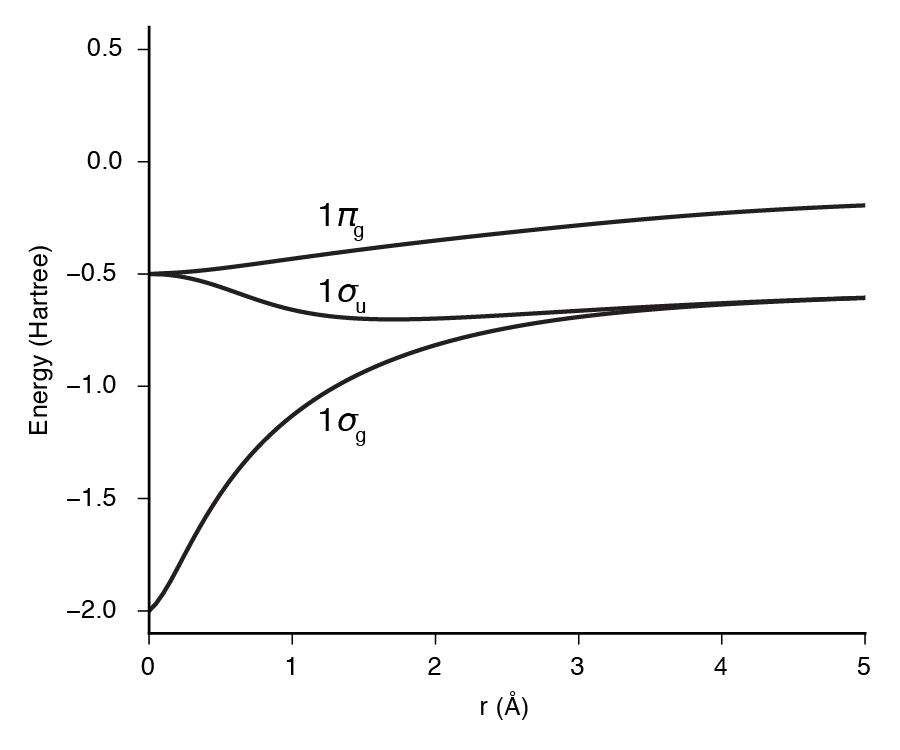
\includegraphics[width=4.5in]{figures/ch2_pec.png}
%   \caption{example caption}
%   \label{fig:example}
%\end{figure}

\section{Avoided crossings}
In this section we discuss some properties of potential energy surfaces. We are particularly interested in understanding when two surfaces become degenerate, because in this circumstances the Born--Oppenheimer approximation is no longer valid.
Consider two electronic states $\tilde{\Phi}_1(\mathbf{R})$ and $\tilde{\Phi}_2(\mathbf{R})$ that are not eigenfunctions of the electronic Hamiltonian. When do the potential energy surfaces obtained by diagonalizing the Hamiltonian in this basis become degenerate? 

Let us write the electronic Hamiltonian in the general\mnote{Here we do not assume that $\tilde{\Phi}_1$ and $\tilde{\Phi}_2$ are eigenfunctions of the Hamiltonian.} basis $\{\tilde{\Phi}_1(\mathbf{R}),\tilde{\Phi}_2(\mathbf{R})\}$ omitting the dependence on the coordinate $\mathbf{R}$
\begin{equation}
\mathbf{H}_\mathrm{el} = 
\begin{pmatrix}
\bra{\tilde{\Phi}_1} \hat{H}_\mathrm{el} \ket{\tilde{\Phi}_1} & \bra{\tilde{\Phi}_1} \hat{H}_\mathrm{el} \ket{\tilde{\Phi}_2}\\
\bra{\tilde{\Phi}_2} \hat{H}_\mathrm{el} \ket{\tilde{\Phi}_1} & \bra{\tilde{\Phi}_2} \hat{H}_\mathrm{el} \ket{\tilde{\Phi}_2}
\end{pmatrix}
=
\begin{pmatrix}
\tilde{E}_{1} & V \\
V^* & \tilde{E}_{2}
\end{pmatrix},
\end{equation}
where we used the fact that the Hamiltonian is Hermitian.\mnote{Because the Hamiltonian is Hermitian we have that $\bra{\tilde{\Phi}_2} \hat{H} \ket{\tilde{\Phi}_1} = \bra{\tilde{\Phi}_1} \hat{H} \ket{\tilde{\Phi}_2}^* =  V^*$.}

The difference between the eigenvalues $E_1$ and $E_2$ of $\mathbf{H}$ is
\begin{equation}
E_2 - E_1 = \sqrt{(\tilde{E}_{1}-\tilde{E}_{2})^2 + 4 |V|^2 }.
\end{equation}
From this equation we deduce that degenerate energy levels require to \textbf{simultaneously} satisfy the conditions:
\begin{align}
\label{eq:molecular_hamiltonian:conical_intersection1}
\tilde{E}_{1}(\mathbf{R}) &= \tilde{E}_{2}(\mathbf{R}), \\
\label{eq:molecular_hamiltonian:conical_intersection2}
|V(\mathbf{R})| &= 0,
\end{align}
that is, the states that form our basis must be degenerate and there should be no coupling.
In general, these two conditions are independent. So suppose we find a point $\mathbf{R}^*$ for which Eqs.\eqref{eq:molecular_hamiltonian:conical_intersection1}-\eqref{eq:molecular_hamiltonian:conical_intersection2} are satisfied, then we can ask what is the dimensionality of the space in which these two states are degenerate?

If we consider a system with $M$ atoms and assume that $|V|$ is not zero for all molecular geometries,\mnote{In other words, $|V|$ is only \textbf{accidentally zero}.} then the subset of molecular geometries for which two potential energy surfaces intersect has dimension $3M - 6 - 2 = 3M - 8$ for non-linear molecules and $3M - 5 - 2 = 3M - 7$ for linear molecules.
%When two electronic state become degenerate in a subspace of molecular geometries we talk about a \textbf{level crossing}.

\begin{example}[Diatomic molecules]
For a diatomic molecule degenerate electronic states live in a $3 \cdot 2 - 7 = -1$ dimensional space.
That is, in general two curves do not cross.
However, if for some reason the coupling $|V| = 0$ for all bond lengths then only one of the two constraints applies.
In this case, degenerate electronic states live in a space of dimension $3 \cdot 2 - 6 = 0$, that is, there may be a finite set of points for which $E_2 = E_1$.
Typical examples of situations when $|V| = 0$ include states with different spin or spatial symmetry.  For example, the singlet and triplet states of H$_2$ are allowed to cross.
Crossings may also occur when two electronic states have different number of electrons.
\end{example}

\section{Nuclear motion on Born--Oppenheimer potential energy surfaces}
Given the eigenvalues and eigenfunctions of the electronic Hamiltonian, it is possible to obtain wave functions for the nuclei by solving the nuclear Schr\"{o}dinger equation:
\begin{equation}
\hat{H}_{{\rm nuc},k} \chi_{v,k}(\mathbf{R}) =  E_{v,k} \chi_{v,k}(\mathbf{R}),
\end{equation}
where $\hat{H}_{{\rm nuc},k}$ is the nuclear Hamiltonian for electronic state $k$:
\begin{equation}
\hat{H}_{{\rm nuc},k} = \hat{T}_{N} + V_{{\rm tot},k}(\mathbf{R}).
\end{equation}
In this approximation the nuclei experience a potential generated by the electrons plus the nuclear-nuclear repulsion:
\begin{equation}
V_{{\rm tot},k}(\mathbf{R}) = \bra{\Phi_k}\hat{H}_{\rm el}(\mathbf{R}) \ket{\Phi_k} + V_{NN}(\mathbf{R}).
\end{equation}
Observations:
\begin{itemize}
\item $\hat{H}_{{\rm nuc},k}$ depends on the electronic state $k$.
\item The electrons react instantaneously to the motion of the nuclei, so the nuclei always see the electrons in a fully relaxed state (adiabatic approximation).
\item This approximation is thus valid when nuclear and electronic motion occur on different time (energy) scales.
\item The first corrections to the BO approximation enter at order $\lambda^6 = \left( \frac{m_e}{M} \right)^{3/2} \approx 1.3 \cdot 10^{-5}$.
\end{itemize}


A large number of interesting and important phenomena are associated with the break down of the adiabatic assumption and require a significantly more refined treatment than the one discussed here.

\end{document}